\chapter{Crochets de Poisson, générateurs et moment cinétique}

\lectureoverview{Le crochet de Poisson est bien plus qu’une manière compacte de réécrire les équations de Hamilton. C’est une opération algébrique qui engendre des transformations. Le crochet avec le Hamiltonien engendre l’évolution temporelle ; le crochet avec la quantité de mouvement engendre les translations ; le crochet avec le moment cinétique engendre les rotations. Dans ce langage, symétrie et conservation deviennent deux lectures d’un même crochet nul. Nous développerons cette idée à partir de l’oscillateur harmonique, puis nous utiliserons l’algèbre du moment cinétique pour obtenir la précession gyroscopique sans introduire les angles d’Euler.}

\section{Fonction le long d’une trajectoire hamiltonienne}

Soit
\[
  F=F(q_1,\ldots,q_n,p_1,\ldots,p_n)
\]
une fonction suffisamment différentiable sur l’espace des phases. On peut la considérer de deux façons. Premièrement, elle associe un nombre à chaque point de l’espace des phases. Deuxièmement, une fois choisie une trajectoire hamiltonienne, elle devient une fonction du temps, puisque le point \((q(t),p(t))\) se déplace. Le long de cette trajectoire,
\begin{equation}
  \frac{dF}{dt}
  =
  \sum_i\left(
    \frac{\partial F}{\partial q_i}\dot q_i
    +\frac{\partial F}{\partial p_i}\dot p_i
  \right).
  \label{eq:l8-chain-rule}
\end{equation}
Les équations de Hamilton,
\begin{equation}
  \dot q_i=\frac{\partial H}{\partial p_i},
  \qquad
  \dot p_i=-\frac{\partial H}{\partial q_i},
  \label{eq:l8-hamilton-equations}
\end{equation}
conduisent à
\begin{equation}
  \frac{dF}{dt}
  =
  \sum_i\left(
    \frac{\partial F}{\partial q_i}
    \frac{\partial H}{\partial p_i}
    -
    \frac{\partial F}{\partial p_i}
    \frac{\partial H}{\partial q_i}
  \right).
  \label{eq:l8-fdot-expanded}
\end{equation}
La combinaison du membre de droite intervient dans toute la mécanique classique, même lorsque aucun de ses deux arguments n’est le Hamiltonien. Cela motive la définition
\begin{equation}
  \boxed{
  \{F,G\}
  =
  \sum_i\left(
    \frac{\partial F}{\partial q_i}
    \frac{\partial G}{\partial p_i}
    -
    \frac{\partial F}{\partial p_i}
    \frac{\partial G}{\partial q_i}
  \right).}
  \label{eq:l8-poisson-definition}
\end{equation}
L’équation~\eqref{eq:l8-fdot-expanded} s’écrit donc
\begin{equation}
  \boxed{\dot F=\{F,H\}.}
  \label{eq:l8-time-generator}
\end{equation}

\begin{classroomqa}
  \audiencequestion{Si l’on remplace le second argument \(H\) par une fonction arbitraire
  \(G\), le crochet donne-t-il toujours la dérivée temporelle de \(F\) ?
  \lecturetimestamp{00:05:45--00:06:15}}
  \lecturerresponse{Non. L’auditoire relève un point important au moment où la notation est généralisée. L’équation~\eqref{eq:l8-poisson-definition} définit \(\{F,G\}\) pour deux fonctions quelconques de l’espace des phases, mais
  \(\dot F=\{F,G\}\) n’est valable que lorsque \(G\) est le Hamiltonien. Une fonction générale \(G\) engendrera une transformation infinitésimale différente.}
\end{classroomqa}

Il est utile d’écrire une petite variation du temps sous la forme
\begin{equation}
  \delta_t F=\epsilon\,\{F,H\}.
  \label{eq:l8-small-time-step}
\end{equation}
Cette forme annonce la suite. L’évolution temporelle est un élément d’une famille plus vaste de transformations engendrées par des crochets de Poisson.

\section{L’algèbre des crochets}

Le crochet peut maintenant servir de calcul à part entière. Ses règles découlent de la différentiation ordinaire :
\begin{align}
  \{A,B\}&=-\{B,A\}, \label{eq:l8-antisymmetry}\\
  \{A+B,C\}&=\{A,C\}+\{B,C\}, \label{eq:l8-additivity}\\
  \{\lambda A,B\}&=\lambda\{A,B\},
    \quad \lambda\ \text{constant}, \label{eq:l8-scalar-rule}\\
  \{AB,C\}&=A\{B,C\}+\{A,C\}B. \label{eq:l8-leibniz}
\end{align}
Ces quatre lignes expriment respectivement l’antisymétrie, l’additivité, la linéarité par rapport à la multiplication par une constante et la règle de Leibniz.
Les fonctions classiques sur l’espace des phases se multiplient de façon commutative ; l’ordre des facteurs ordinaires \(A\) et \(B\) dans la dernière ligne est donc sans importance. Ce ne sera plus vrai pour les opérateurs en mécanique quantique. L’antisymétrie implique aussi
\begin{equation}
  \{A,A\}=0.
  \label{eq:l8-self-bracket}
\end{equation}

Pour les coordonnées canoniques, les crochets élémentaires sont
\begin{equation}
  \boxed{
  \{q_i,q_j\}=0,\qquad
  \{p_i,p_j\}=0,\qquad
  \{q_i,p_j\}=\delta_{ij}.}
  \label{eq:l8-canonical-brackets}
\end{equation}
Toute fonction dépendant uniquement de \(q_i\) a un crochet nul avec toute autre fonction dépendant uniquement de \(q_i\) ; la même propriété vaut pour les fonctions dépendant uniquement de \(p_i\). Un crochet non nul exige qu’une coordonnée canonique rencontre sa quantité de mouvement conjuguée. Le symbole de Kronecker dans l’équation~\eqref{eq:l8-canonical-brackets} indique que seuls les indices correspondants se combinent.

\subsection{L’oscillateur harmonique comme cas d’essai}

Considérons
\begin{equation}
  H=\frac{p^2}{2m}+\frac{kq^2}{2}.
  \label{eq:l8-oscillator-hamiltonian}
\end{equation}
Nous n’utilisons maintenant délibérément que les règles des crochets et l’équation~\eqref{eq:l8-time-generator}. D’abord,
\begin{align}
  \dot q
  &=\{q,H\}\\
  &=\frac{1}{2m}\{q,p^2\}\\
  &=\frac{1}{2m}\left(p\{q,p\}+\{q,p\}p\right)\\
  &=\frac{p}{m}.
  \label{eq:l8-qdot-oscillator}
\end{align}
Le terme de potentiel disparaît parce que \(\{q,q^2\}=0\). De même,
\begin{align}
  \dot p
  &=\{p,H\}\\
  &=\frac{k}{2}\{p,q^2\}\\
  &=\frac{k}{2}\left(q\{p,q\}+\{p,q\}q\right)\\
  &=-kq.
  \label{eq:l8-pdot-oscillator}
\end{align}
Le signe moins vient précisément de l’antisymétrie
\(\{p,q\}=-\{q,p\}=-1\). En combinant les deux équations du premier ordre, on obtient
\begin{equation}
  m\ddot q=-kq.
  \label{eq:l8-hooke-equation}
\end{equation}

\begin{figure}[htbp]
  \centering
  
\includegraphics[width=0.82\textwidth]{lecture_08_figure_01.png}
  \caption{Le Hamiltonien de l’oscillateur et les deux calculs de crochets qui donnent \(\dot q=p/m\) et \(\dot p=-kq\).}
  \lectureframe{00:23:20}
\end{figure}

Pendant le calcul, la classe cherche un verbe signifiant
\emph{prendre un crochet de Poisson} et opte provisoirement pour
\emph{poissonner}. Cette plaisanterie marque un véritable changement de point de vue : une fois l’algèbre connue, on peut l’utiliser directement au lieu de redériver chaque résultat à partir de la définition.

\begin{classroomqa}
  \audiencequestion{Cette structure mathématique est-elle un groupe ou une algèbre ?
  Possède-t-elle des inverses ? \lecturetimestamp{00:23:48--00:24:16}}
  \lecturerresponse{Ce n’est pas un groupe : l’opération de crochet ne fournit ni l’élément neutre ni les inverses requis. Les fonctions sur l’espace des phases forment une algèbre de Poisson : elles sont munies de l’addition et de la multiplication commutatives ordinaires, ainsi que d’un crochet antisymétrique qui satisfait à la règle de Leibniz. Une identité supplémentaire, l’identité de Jacobi, complète la définition abstraite usuelle, mais elle n’est pas développée dans ce cours.}
\end{classroomqa}

\begin{classroomqa}
  \audiencequestion{Quel est le lien entre les crochets de Poisson et les commutateurs quantiques ? \lecturetimestamp{00:24:18--00:25:00}}
  \lecturerresponse{Le cours n’en donne qu’un aperçu. Lors du passage à la mécanique quantique, le crochet classique est remplacé, schématiquement, par
  \[
    \{A,B\}_{\mathrm{PB}}
    \longleftrightarrow
    \frac{1}{i\hbar}[\widehat A,\widehat B].
  \]
Cette correspondance appelle des réserves concernant l’ordre des opérateurs et la quantification ; elle n’est pas utilisée ici comme un théorème.}
\end{classroomqa}

Pour l’oscillateur, le crochet n’a fait que retrouver les équations de Hamilton. Son véritable intérêt apparaît lorsque le générateur est une quantité conservée autre que \(H\).

\section{Retrouver le moment cinétique à partir de la symétrie de rotation}

Rappelons la forme infinitésimale de la construction de Noether utilisée plus tôt dans le cours. Si une symétrie continue modifie les coordonnées selon
\begin{equation}
  \delta q_i=\epsilon F_i(q),
  \label{eq:l8-noether-variation}
\end{equation}
alors, dans le cadre considéré ici, la quantité conservée est
\begin{equation}
  G=\sum_i p_iF_i(q).
  \label{eq:l8-noether-charge}
\end{equation}
On peut omettre le facteur global \(\epsilon\) : multiplier une quantité conservée par un nombre fixe ne change pas la loi de conservation.

Prenons une particule et effectuons une rotation infinitésimale autour de l’axe \(z\). Avec l’orientation utilisée dans le cours,
\begin{equation}
  \delta x=-\epsilon y,\qquad
  \delta y=\epsilon x,\qquad
  \delta z=0.
  \label{eq:l8-z-rotation}
\end{equation}
L’équation~\eqref{eq:l8-noether-charge} donne
\begin{equation}
  L_z=-p_xy+p_yx=xp_y-yp_x.
  \label{eq:l8-lz}
\end{equation}
En permutant cycliquement \(x\), \(y\) et \(z\),
\begin{equation}
  \boxed{\begin{aligned}
    L_x&=yp_z-zp_y,\\
    L_y&=zp_x-xp_z,\\
    L_z&=xp_y-yp_x.
  \end{aligned}}
  \label{eq:l8-angular-components}
\end{equation}
Ce sont les composantes de
\begin{equation}
  \boldsymbol L=\boldsymbol r\times\boldsymbol p.
  \label{eq:l8-cross-product}
\end{equation}

\begin{figure}[htbp]
  \centering
  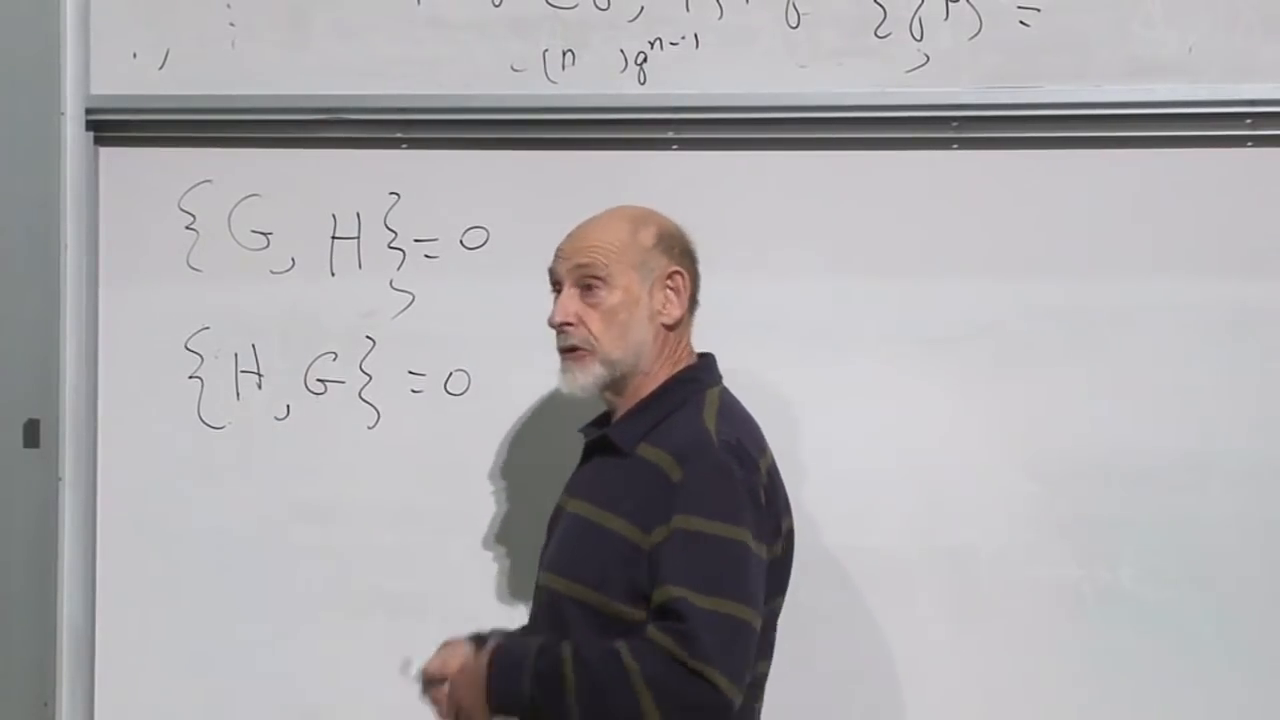
\includegraphics[width=0.82\textwidth]{lecture_08_figure_02.png}
  \caption{Les trois composantes cartésiennes du moment cinétique et leur forme compacte en produit vectoriel.}
  \lectureframe{00:34:00}
\end{figure}

Une rotation autour d’un vecteur unitaire arbitraire \(\boldsymbol n\) est engendrée par
\begin{equation}
  L_{\boldsymbol n}=\boldsymbol n\cdot\boldsymbol L.
  \label{eq:l8-arbitrary-axis}
\end{equation}
Pour un système isolé invariant par rotation, les trois composantes sont conservées. Si seules les rotations autour d’un axe restent des symétries, seule la composante selon cet axe est nécessairement conservée.

\section{Le moment cinétique engendre les rotations}

Au lieu de résoudre tout de suite un problème de dynamique de rotation, examinons ce que \(L_z\) donne sous l’action du crochet. En utilisant
l’équation~\eqref{eq:l8-lz},
\begin{align}
  \{x,L_z\}
  &=\{x,xp_y-yp_x\}
   =-y\{x,p_x\}
   =-y,\\
  \{y,L_z\}
  &=\{y,xp_y-yp_x\}
   =x\{y,p_y\}
   =x,\\
  \{z,L_z\}&=0.
  \label{eq:l8-position-rotation-brackets}
\end{align}
Ce sont exactement les coefficients de l’équation~\eqref{eq:l8-z-rotation}.

\begin{figure}[htbp]
  \centering
  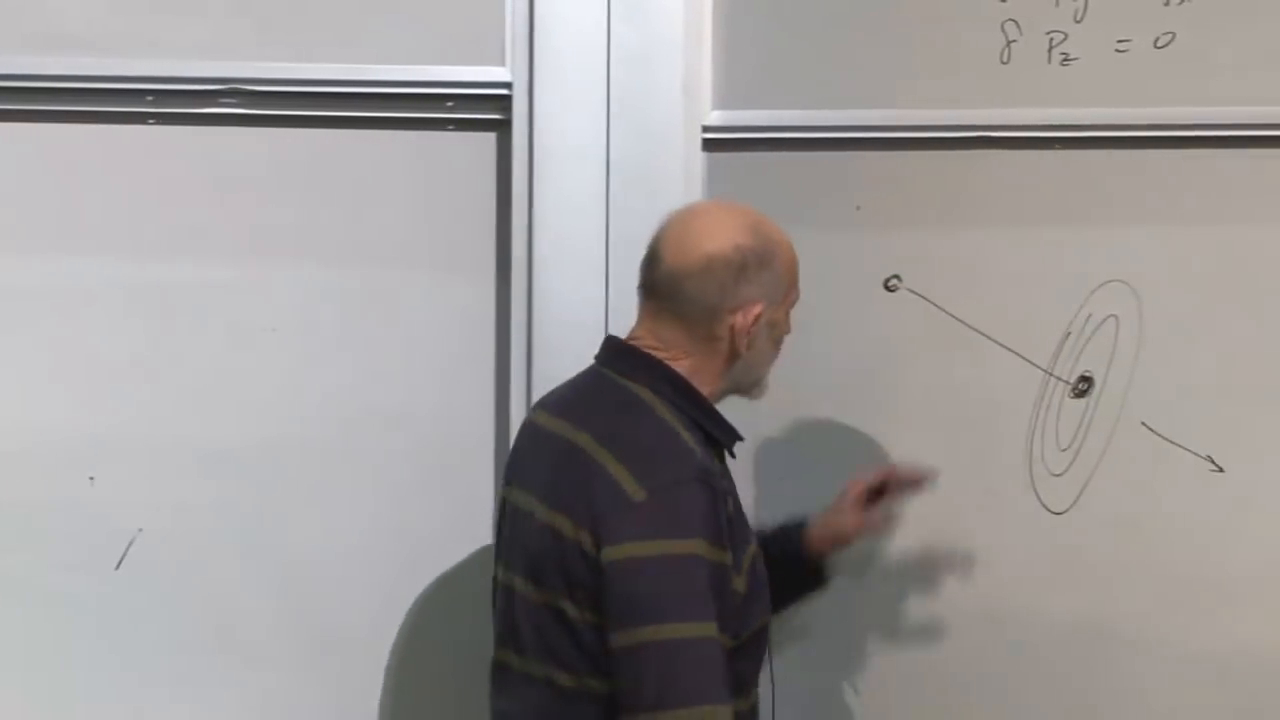
\includegraphics[width=0.82\textwidth]{lecture_08_figure_03.png}
  \caption{Crochets des coordonnées avec \(L_z\) : le crochet reproduit la rotation infinitésimale de \((x,y,z)\).}
  \lectureframe{00:38:41}
\end{figure}

La quantité de mouvement est elle aussi un vecteur, et le même calcul donne
\begin{equation}
  \begin{aligned}
    \{p_x,L_z\}&=-p_y,\\
    \{p_y,L_z\}&=p_x,\\
    \{p_z,L_z\}&=0.
  \end{aligned}
  \label{eq:l8-momentum-rotation-brackets}
\end{equation}

\begin{figure}[htbp]
  \centering
  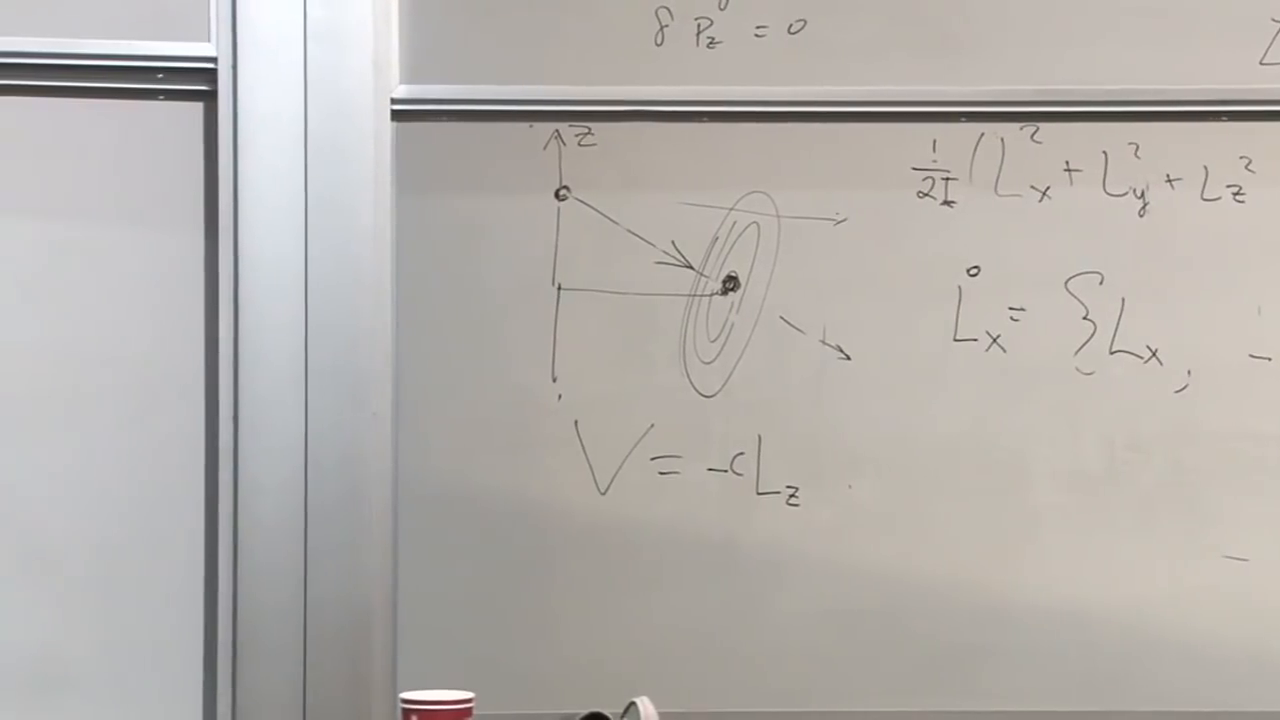
\includegraphics[width=0.82\textwidth]{lecture_08_figure_04.png}
  \caption{La position et la quantité de mouvement suivent le même schéma vectoriel sous la rotation engendrée par \(L_z\).}
  \lectureframe{00:42:08}
\end{figure}

La relation hamiltonienne générale s’écrit donc
\begin{equation}
  \boxed{\delta_G A=\epsilon\{A,G\}.}
  \label{eq:l8-generator-rule}
\end{equation}
Toute fonction de l’espace des phases \(G\) définit une telle transformation canonique infinitésimale. Si \(G=L_z\), c’est une rotation. Si \(G=H\), c’est un petit pas dans le temps.

\begin{classroomqa}
  \audiencequestion{Le cours parle parfois de faire tourner le système et parfois de faire tourner les coordonnées. Quelle convention utilise-t-on dans les équations avec les crochets ? \lecturetimestamp{00:28:22--00:29:35}}
  \lecturerresponse{L’équation~\eqref{eq:l8-z-rotation} fixe la convention : il s’agit de la rotation active infinitésimale
  \((x,y)\mapsto(x-\epsilon y,y+\epsilon x)\). Une rotation passive des axes donne le signe opposé. Une fois la convention fixée, les formules avec les crochets ne présentent aucune ambiguïté.}
\end{classroomqa}

\section{La quantité de mouvement engendre les translations}

Une translation suivant une coordonnée s’écrit
\begin{equation}
  \delta q=\epsilon.
  \label{eq:l8-q-translation}
\end{equation}
Ici, \(F(q)=1\) dans l’équation~\eqref{eq:l8-noether-variation}, donc la quantité conservée correspondante est \(p\). La propriété de générateur prédit
\begin{equation}
  \{f(q),p\}=\frac{df}{dq}.
  \label{eq:l8-translation-derivative}
\end{equation}
Le cours démontre d’abord ce résultat pour les puissances, par récurrence. Le cas de base est
\(\{q,p\}=1\). Supposons que
\begin{equation}
  \{q^{n-1},p\}=(n-1)q^{n-2}.
  \label{eq:l8-induction-hypothesis}
\end{equation}
La règle du produit donne alors
\begin{align}
  \{q^n,p\}
  &=\{q\,q^{n-1},p\}\\
  &=q\{q^{n-1},p\}+\{q,p\}q^{n-1}\\
  &=(n-1)q^{n-1}+q^{n-1}\\
  &=nq^{n-1}.
  \label{eq:l8-power-translation}
\end{align}
La linéarité étend le résultat aux polynômes et aux développements en séries entières convergentes. Plus directement, la définition du crochet donne l’équation~\eqref{eq:l8-translation-derivative} pour toute fonction différentiable \(f(q)\) :
\begin{equation}
  \{f(q),p\}
  =
  \frac{\partial f}{\partial q}
  \frac{\partial p}{\partial p}
  =f'(q).
\end{equation}

\begin{figure}[htbp]
  \centering
  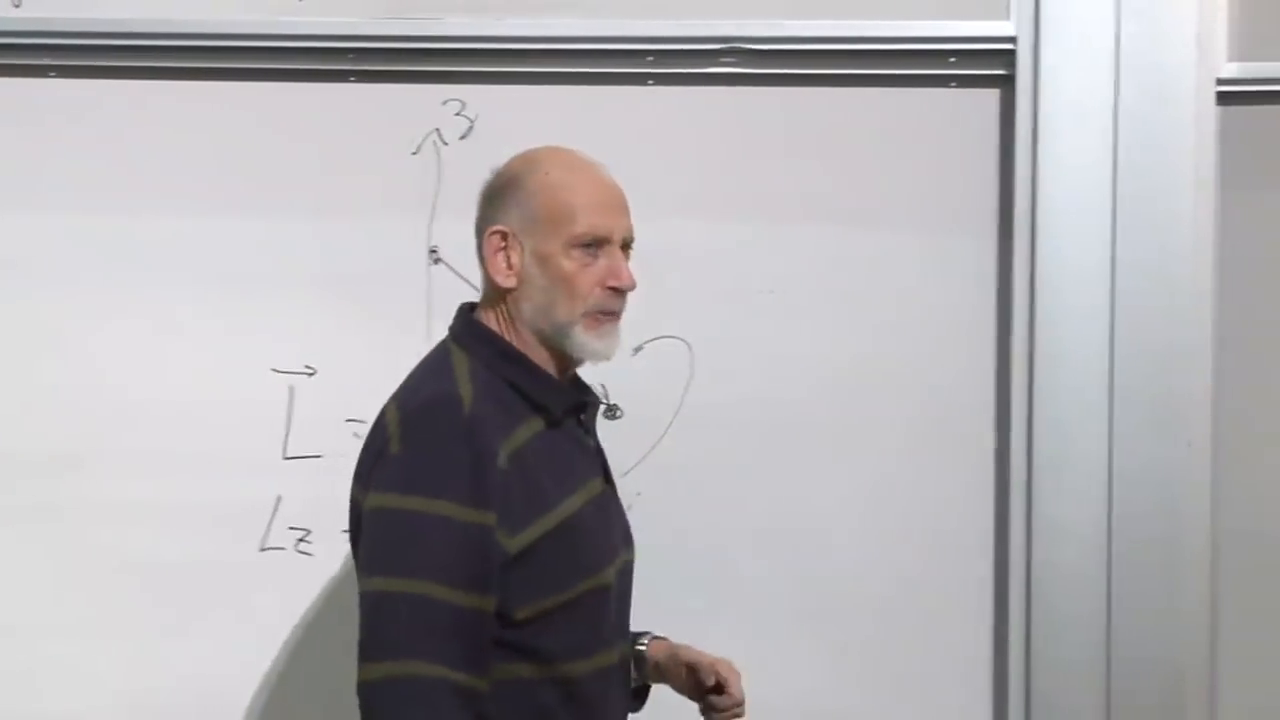
\includegraphics[width=0.82\textwidth]{lecture_08_figure_05.png}
  \caption{Le résultat sur les translations après la démonstration par récurrence : \(\{F(q),p\}=dF/dq\).}
  \lectureframe{00:53:18}
\end{figure}

Nous avons maintenant vu trois manifestations d’une même idée :
\begin{center}
  \begin{tabular}{@{}>{\raggedright\arraybackslash}p{0.37\textwidth}
                      >{\raggedright\arraybackslash}p{0.55\textwidth}@{}}
    \toprule
    Générateur et transformation & Action infinitésimale\\
    \midrule
    \(H\), translation temporelle & \(\delta_tA=\epsilon\{A,H\}\)\\
    \(p_i\), translation spatiale & \(\delta A=\epsilon\{A,p_i\}\)\\
    \(L_i\), rotation & \(\delta A=\epsilon\{A,L_i\}\)\\
    \bottomrule
  \end{tabular}
\end{center}
La quantité conservée associée à une symétrie continue est aussi le générateur de cette symétrie.

\section{Un crochet, deux interprétations}

Soit \(G(q,p)\) un générateur proposé. S’il est conservé et ne dépend pas explicitement du temps, alors
\begin{equation}
  \dot G=\{G,H\}=0.
  \label{eq:l8-g-conserved}
\end{equation}
Par antisymétrie,
\begin{equation}
  \{H,G\}=0.
  \label{eq:l8-h-invariant}
\end{equation}
Les équations sont mathématiquement équivalentes, mais leurs interprétations physiques diffèrent :
\begin{itemize}
  \item \(\{G,H\}=0\) signifie que \(G\) ne varie pas au cours de l’évolution temporelle engendrée par \(H\).
  \item \(\{H,G\}=0\) signifie que \(H\) ne varie pas sous la transformation engendrée par \(G\).
\end{itemize}
La première est une loi de conservation ; la seconde, une symétrie du Hamiltonien. Le lien de Noether se trouve condensé dans un zéro.

\begin{figure}[htbp]
  \centering
  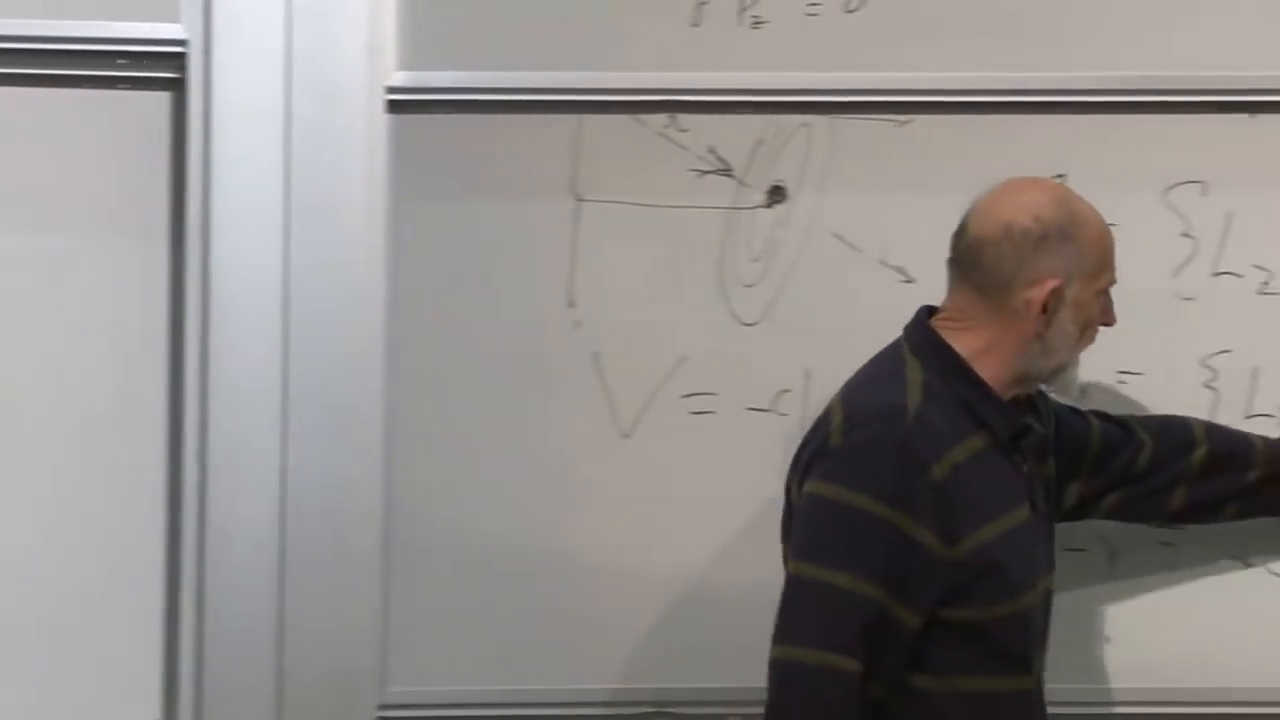
\includegraphics[width=0.82\textwidth]{lecture_08_figure_06.png}
  \caption{Les deux ordres d’un même crochet nul : conservation de \(G\) et invariance de \(H\) sous la transformation engendrée par \(G\).}
  \lectureframe{01:03:05}
\end{figure}

\begin{classroomqa}
  \audiencequestion{Si l’on connaît une quantité conservée, peut-on toujours retrouver la symétrie associée ? \lecturetimestamp{01:01:42--01:02:15}}
  \lecturerresponse{Dans ce cadre hamiltonien, oui : prenons le crochet de chaque variable de l’espace des phases avec \(G\). L’ensemble \(\delta_GA=\epsilon\{A,G\}\) indique comment les variables se transforment. Par exemple, les crochets avec \(L_z\) révèlent une rotation, même si cette interprétation n’était pas connue au départ. Des subtilités globales et liées aux frontières peuvent intervenir dans des cadres plus avancés, mais c’est l’énoncé infinitésimal local qui est utilisé ici.}
\end{classroomqa}

\begin{classroomqa}
  \audiencequestion{Ces équations avec les crochets nous indiquent-elles le mouvement physique à l’origine de la loi de conservation ?
  \lecturetimestamp{00:56:01--00:58:13}}
  \lecturerresponse{Non. Elles identifient la transformation de symétrie, et non la trajectoire réelle. La conservation de \(L_z\) indique une symétrie de rotation ; elle ne signifie pas que la particule décrit un cercle. L’évolution temporelle réelle est engendrée par \(H\). Un crochet avec un autre générateur décrit une autre direction de transformation dans l’espace des phases.}
\end{classroomqa}

\begin{classroomqa}
  \audiencequestion{Existe-t-il un énoncé général sur les transformations qui ne suppose pas déjà la conservation ? \lecturetimestamp{01:02:40--01:04:45}}
  \lecturerresponse{Oui. L’équation~\eqref{eq:l8-generator-rule} définit une transformation infinitésimale pour toute fonction \(G\), qu’elle soit conservée ou non. Elle ne devient une symétrie que lorsque le Hamiltonien est invariant : \(\{H,G\}=0\). Lue dans l’ordre inverse, la même condition indique alors que \(G\) est conservé.}
\end{classroomqa}

\section{L’algèbre du moment cinétique}

Le calcul qui suit nous évite d’entraîner les coordonnées de la particule dans chaque problème de rotation. Commençons par
\[
  L_x=yp_z-zp_y,\qquad
  L_z=xp_y-yp_x.
\]
Dans \(\{L_x,L_z\}\), la plupart des termes croisés s’annulent parce que leurs indices ne forment pas des paires canoniques. Les contractions restantes donnent
\begin{align}
  \{L_x,L_z\}
  &=\{yp_z-zp_y,xp_y-yp_x\}\\
  &=xp_z-zp_x\\
  &=-L_y.
  \label{eq:l8-lx-lz}
\end{align}
Inverser l’ordre supprime le signe moins. La permutation cyclique des coordonnées donne
\begin{equation}
  \boxed{\begin{aligned}
    \{L_x,L_y\}&=L_z,\\
    \{L_y,L_z\}&=L_x,\\
    \{L_z,L_x\}&=L_y.
  \end{aligned}}
  \label{eq:l8-angular-algebra}
\end{equation}
En notation indicielle,
\begin{equation}
  \{L_i,L_j\}=\varepsilon_{ijk}L_k.
  \label{eq:l8-angular-algebra-index}
\end{equation}

\begin{figure}[htbp]
  \centering
  \includegraphics[width=0.82\textwidth]{lecture_08_figure_07.png}
  \caption{L’algèbre cyclique des crochets de Poisson des trois composantes du moment cinétique.}
  \lectureframe{01:10:52}
\end{figure}

On aurait aussi pu prévoir le résultat. Puisque \(\boldsymbol L\) est un vecteur, le crochet de sa composante selon \(x\) avec \(L_z\) doit donner la variation infinitésimale de cette composante sous une rotation autour de \(z\), soit \(-L_y\). Le calcul explicite confirme cet argument géométrique. Ces équations sont aussi les précurseurs classiques des relations de commutation quantiques du moment cinétique.

\section{Un gyroscope à rotation rapide}

À titre d’application, considérons un gyroscope : un volant d’inertie en rotation rapide, dont le centre se trouve à une distance fixe \(R\) d’un pivot. Soit \(\boldsymbol r\) le vecteur allant du pivot au centre du volant. Celui-ci tourne si rapidement autour de son axe que son moment cinétique dominant reste aligné avec cette direction. Dans l’approximation utilisée dans le cours,
\begin{equation}
  \boldsymbol L=\ell\,\boldsymbol r,
  \qquad
  L_z=\ell z,
  \label{eq:l8-L-parallel-r}
\end{equation}
où \(\ell=L/R\) est considéré comme constant. On néglige d’abord les moments cinétiques plus faibles associés à la nutation ou au mouvement de l’axe.

\begin{figure}[htbp]
  \centering
  \begin{tikzpicture}[scale=0.95,>=Latex]
    \coordinate (P) at (0,3.2);
    \coordinate (C) at (3.7,1.55);
    \draw[->] (0,-0.2) -- (0,4.35) node[above] {\(z\)};
    \fill (P) circle (1.7pt) node[left] {pivot};
    \draw[very thick,->] (P) -- (C)
      node[midway,above right] {\(\boldsymbol r\parallel\boldsymbol L\)};
    \fill (C) circle (1.7pt);
    \draw[dashed] (P) -- (0,1.55);
    \draw[dashed] (0,1.55) -- (C);
    \node[left] at (0,1.55) {\(z\)};
    \begin{scope}[shift={(C)},rotate=-24]
      \draw[very thick] (0,0) ellipse (0.65 and 1.35);
      \draw[thick] (0,0) ellipse (0.42 and 0.9);
    \end{scope}
    \draw[->,thick] (2.15,2.85)
      arc[start angle=140,end angle=35,radius=1.65];
  \end{tikzpicture}
  \caption{Approximation du gyroscope à rotation rapide. La distance entre le pivot et le centre est fixe, et le moment cinétique dominant dû à la rotation reste aligné avec l’axe et \(\boldsymbol r\).}
\end{figure}

\begin{figure}[htbp]
  \centering
  \includegraphics[width=0.82\textwidth]{lecture_08_figure_08.png}
  \caption{Schéma au tableau du volant d’inertie, avec \(H_{\rm rot}=L^2/(2I)\), et annulation qui démontre la conservation de \(\boldsymbol L\) en l’absence de couple.}
  \lectureframe{01:18:54}
\end{figure}

\subsection{Sans gravité : pourquoi chaque composante reste constante}

Pour le rotor axialement symétrique simplifié,
\begin{equation}
  H_{\mathrm{rot}}
  =\frac{1}{2I}
  \left(L_x^2+L_y^2+L_z^2\right)
  =\frac{L^2}{2I}.
  \label{eq:l8-rotational-hamiltonian}
\end{equation}
Le coefficient est \(1/(2I)\), et non \(I/2\) ; cette erreur est commise puis corrigée au tableau. En utilisant l’équation~\eqref{eq:l8-angular-algebra},
\begin{align}
  \dot L_x
  &=\{L_x,H_{\mathrm{rot}}\}\\
  &=\frac{1}{2I}\left(
    2L_y\{L_x,L_y\}
    +2L_z\{L_x,L_z\}
  \right)\\
  &=\frac{1}{I}\left(L_yL_z-L_zL_y\right)=0.
  \label{eq:l8-free-lx}
\end{align}
Par permutation cyclique,
\begin{equation}
  \dot L_x=\dot L_y=\dot L_z=0.
  \label{eq:l8-free-angular-momentum}
\end{equation}
Le scalaire \(L^2\) a un crochet nul avec chaque composante \(L_i\) ; dans le langage de cette algèbre, c’est un invariant de Casimir. Ainsi, en l’absence de couple, le gyroscope conserve à la fois la norme et la direction de son moment cinétique.

\begin{classroomqa}
  \audiencequestion{Le moment d’inertie n’est-il qu’un nombre ici ?
  \lecturetimestamp{01:14:23--01:15:05}}
  \lecturerresponse{Pour ce modèle réduit, oui. Il encode la distribution de masse du volant autour de son axe de rotation. Un solide général possède un tenseur d’inertie et un Hamiltonien de rotation
  \(\sum_i L_i^2/(2I_i)\) dans ses axes principaux. Le cours choisit le rotor symétrique à rotation rapide, plus simple, car l’objectif est de présenter la méthode des crochets de Poisson plutôt que de développer la dynamique complète d’un solide.}
\end{classroomqa}

\subsection{Gravité et signe du potentiel}

Prenons la coordonnée verticale \(z\) orientée vers le haut et plaçons le pivot à l’origine. L’énergie potentielle gravitationnelle du centre du volant est
\begin{equation}
  V=Mgz.
  \label{eq:l8-mgz}
\end{equation}
Puisque \(L_z=\ell z\),
\begin{equation}
  V=cL_z,
  \qquad
  c=\frac{Mg}{\ell}=\frac{MgR}{L}.
  \label{eq:l8-potential-lz}
\end{equation}
Ici, \(c>0\) lorsque \(\boldsymbol L\) est choisi parallèle à \(\boldsymbol r\). Si le volant tourne en sens opposé, la relation signée entre \(\boldsymbol L\) et \(\boldsymbol r\) s’inverse, ainsi que la fréquence de précession correspondante avec son signe.

\begin{figure}[htbp]
  \centering
  \includegraphics[width=0.82\textwidth]{lecture_08_figure_09.png}
  \caption{Géométrie à longueur fixe à l’origine de \(\boldsymbol L=\ell\boldsymbol r\) et de \(L_z=\ell z\).}
  \lectureframe{01:25:38}
\end{figure}

\begin{figure}[htbp]
  \centering
  \includegraphics[width=0.82\textwidth]{lecture_08_figure_10.png}
  \caption{Une étape intermédiaire du tableau montre \(V=-cL_z\). Le signe est corrigé plus tard, une fois \(z\) fixé vers le haut : avec \(\boldsymbol L=\ell\boldsymbol r\) et \(\ell>0\), le résultat cohérent est \(V=+cL_z\).}
  \lectureframe{01:22:43}
\end{figure}

\begin{classroomqa}
  \audiencequestion{Pourquoi peut-on remplacer la hauteur par une composante du moment cinétique ? La ligne oblique représente-t-elle un axe ou un vecteur position ?
  \lecturetimestamp{01:22:20--01:25:43}}
  \lecturerresponse{Il vaut mieux désigner la ligne oblique par \(\boldsymbol r\), le vecteur allant du pivot fixe au centre du volant. Un axe physique peut lui être parallèle, mais la relation utilisée dans le calcul est l’approximation de rotation rapide
  \(\boldsymbol L=\ell\boldsymbol r\). Leurs composantes selon \(z\) sont donc proportionnelles. Au fil de la discussion, les étiquettes changent plusieurs fois avant que cette distinction soit établie.}
\end{classroomqa}

\begin{classroomqa}
  \audiencequestion{Quelles hypothèses permettent de considérer \(\ell\) comme constant, et que se passe-t-il si le centre du volant peut glisser radialement ?
  \lecturetimestamp{01:25:43--01:26:38,\allowbreak\ 01:34:22--01:35:00}}
  \lecturerresponse{On suppose que la rotation dominante est beaucoup plus importante que le moment cinétique associé au mouvement lent, et que la distance entre le pivot et le centre est fixe. La norme du moment cinétique de rotation varie alors peu et \(\boldsymbol L\) tourne avec \(\boldsymbol r\). Si le centre pouvait glisser radialement, \(z\) ne serait plus proportionnel à \(L_z\) selon un coefficient constant unique ; le Hamiltonien réduit \(V=cL_z\) ne décrirait donc plus le mouvement.}
\end{classroomqa}

\begin{classroomqa}
  \audiencequestion{Pourquoi le tableau montre-t-il d’abord un signe moins, puis un signe plus ? Le sens de rotation compte-t-il ?
  \lecturetimestamp{01:27:13--01:28:15,\allowbreak\ 01:33:09--01:33:21}}
  \lecturerresponse{Le signe initial résulte d’une erreur faite au tableau et d’une convention d’axe qui n’était pas encore fixée. Une fois \(z\) défini vers le haut, \(V=Mgz\) augmente avec la hauteur. Si \(\boldsymbol L=\ell\boldsymbol r\) avec \(\ell>0\), on obtient \(V=+cL_z\). Inverser le sens de rotation inverse la proportionnalité signée et le sens de la précession, mais ne rétablit pas un choix de signe arbitraire.}
\end{classroomqa}

\subsection{La précession en trois équations courtes}

Le Hamiltonien réduit complet est
\begin{equation}
  H=
  \frac{1}{2I}\left(L_x^2+L_y^2+L_z^2\right)+cL_z.
  \label{eq:l8-full-gyro-hamiltonian}
\end{equation}
Nous avons déjà montré que \(L^2\) a un crochet nul avec chaque \(L_i\). Seul le terme linéaire contribue :
\begin{align}
  \dot L_z&=\{L_z,H\}=0,\\
  \dot L_x&=\{L_x,H\}=c\{L_x,L_z\}=-cL_y,\\
  \dot L_y&=\{L_y,H\}=c\{L_y,L_z\}=cL_x.
  \label{eq:l8-precession-equations}
\end{align}

\begin{figure}[htbp]
  \centering
  \includegraphics[width=0.82\textwidth]{lecture_08_figure_11.png}
  \caption{Les équations finales pour les composantes : \(L_z\) reste constant, tandis que \(L_x\) et \(L_y\) tournent l’un en l’autre.}
  \lectureframe{01:30:35}
\end{figure}

La composante verticale et la norme de la composante horizontale sont constantes :
\begin{equation}
  \frac{d}{dt}(L_x^2+L_y^2)
  =2L_x(-cL_y)+2L_y(cL_x)=0.
\end{equation}
En combinant les composantes horizontales,
\begin{equation}
  L_+=L_x+iL_y,
  \qquad
  \dot L_+=icL_+,
\end{equation}
on obtient
\begin{equation}
  L_+(t)=L_+(0)e^{ict}.
  \label{eq:l8-precession-solution}
\end{equation}
Le vecteur moment cinétique précesse donc autour de l’axe vertical à la vitesse angulaire \(|c|=MgR/L\). Son inclinaison reste constante dans ce mouvement régulier idéalisé.

\begin{classroomqa}
  \audiencequestion{Le terme d’énergie de rotation a-t-il été négligé dans l’écriture des équations de précession ?
  \lecturetimestamp{01:35:01--01:35:49}}
  \lecturerresponse{Non. Il fait partie du Hamiltonien complet, comme dans l’équation~\eqref{eq:l8-full-gyro-hamiltonian}. Il ne contribue tout simplement pas à \(\dot L_i\), car \(\{L_i,L^2\}=0\), annulation déjà démontrée dans le calcul sans couple. La question de l’étudiant explicite cette étape implicite.}
\end{classroomqa}

\begin{classroomqa}
  \audiencequestion{La précession uniforme est-elle un équilibre ? Que se passe-t-il après une petite impulsion ? \lecturetimestamp{01:32:38--01:33:08}}
  \lecturerresponse{Il vaut mieux parler d’un mouvement régulier ou stationnaire que d’un équilibre statique. Une petite impulsion ajoute en général une nutation, c’est-à-dire une oscillation de l’angle d’inclinaison. Pour un volant en rotation très rapide, cette oscillation est faible, ce qui explique pourquoi le traitement réduit ne retient qu’une précession presque uniforme.}
\end{classroomqa}

\begin{classroomqa}
  \audiencequestion{La précession exige-t-elle un support ou un axe réel ?
  \lecturetimestamp{01:31:49--01:32:38,\allowbreak\ 01:33:49--01:35:00}}
  \lecturerresponse{Ce modèle mécanique suppose que la distance entre le pivot et le centre est fixe ; une contrainte doit donc assurer le support. Le résultat algébrique plus général est le suivant : chaque fois qu’un terme du Hamiltonien est linéaire en une composante du moment cinétique, la même algèbre des crochets produit une précession. La source microscopique du moment cinétique n’a pas besoin d’être une véritable roue montée sur un axe.}
\end{classroomqa}

\begin{classroomqa}
  \audiencequestion{Est-ce la même précession que celle du spin de l’électron ou du noyau dans un champ magnétique, ou que celle de l’orbite d’une planète ?
  \lecturetimestamp{01:35:50--01:37:00}}
  \lecturerresponse{Un moment magnétique couplé à un champ magnétique possède un Hamiltonien linéaire en une composante du spin et obéit donc à la même algèbre du moment cinétique. La précession du spin nucléaire est au fondement de la résonance magnétique nucléaire. La précession du périhélie d’une orbite planétaire est un phénomène différent qui partage par hasard le mot \emph{précession} ; le calcul n’est pas le même.}
\end{classroomqa}

\begin{classroomqa}
  \audiencequestion{Le gyroscope monté latéralement est-il essentiellement le même objet qu’une toupie ? \lecturetimestamp{01:37:02--01:37:23}}
  \lecturerresponse{Oui. La distinction relève surtout du vocabulaire géométrique : lorsque l’axe de rotation s’étend latéralement depuis son support, on parle généralement de gyroscope ; lorsqu’il est presque vertical, on parle de toupie. La structure du moment cinétique et du couple est la même.}
\end{classroomqa}

\section{Ce que le calcul a permis d’établir}

Nous n’avons introduit aucun angle d’Euler ni suivi les coordonnées de chaque élément de la roue. Une fois que
\[
  \{L_i,L_j\}=\varepsilon_{ijk}L_k
\]
était connue, les équations des variables qui nous intéressent en ont découlé directement. C’est là la démonstration de puissance visée. L’oscillateur a montré que les crochets de Poisson peuvent reproduire une dynamique familière. Le moment cinétique a montré qu’ils permettent bien davantage :
\begin{itemize}
  \item une quantité conservée engendre la symétrie infinitésimale qui lui est associée ;
  \item la conservation de \(G\) et l’invariance de \(H\) sont les deux interprétations de \(\{G,H\}=0\) ;
  \item l’algèbre des observables peut se refermer sur elle-même, ce qui permet de résoudre la dynamique sans revenir aux coordonnées microscopiques ;
  \item un Hamiltonien linéaire en une composante du moment cinétique produit une précession autour de cet axe.
\end{itemize}
Le cours s’arrête avant les équations d’Euler complètes d’un solide général. Sa conclusion, plus limitée, est déjà complète : les bons générateurs et leur algèbre de Poisson mettent en évidence à la fois la symétrie et le mouvement avec une remarquable économie.
